\section{Applications}

\subsection{Denoising}

\begin{description}
 \item[btkNLMDenoising] This program applies a non-local mean filter to a 3D image for denoising purpose. Usage: \texttt{-i input\_image\_filename -o output\_image\_filename}. The best results are usually obtained by using a mask (or a padding value).
\end{description}

\begin{description}
 \item[btkNLMDenoising4DImage] This program applies a non-local mean filter to each 3D image of a 4D image, for denoising purpose. Usage: \texttt{-i input\_image\_filename -o output\_image\_filename}. The best results are usually obtained by using a mask (or a padding value).
\end{description}


\subsection{Anatomical reconstruction}

\begin{description}
 \item[btkImageReconstruction] This program allows to obtain a
high-resolution image from a set of low-resolution images, typically
axial, coronal, and sagital acquisitions~\cite{Rousseau2006}. \\\\
Minimal usage: \texttt{btkImageReconstruction -i image1 $\cdots$ -i imageN -o
output}. 

Recommended usage: \texttt{btkImageReconstruction -i image1 $\cdots$ -i imageN
-m mask1 $\cdots$ -m maskN -o output --mask}. The use of a mask provide
better results since it allows an accuratelly estimation of the initial
transform, and constrains the registration to the region of interest.

The full list of optional parameters of the method can be obtained by
\texttt{btkImageReconstruction --help}

\end{description}

\begin{figure}[t]
\centering
\begin{tabular}{ccc}
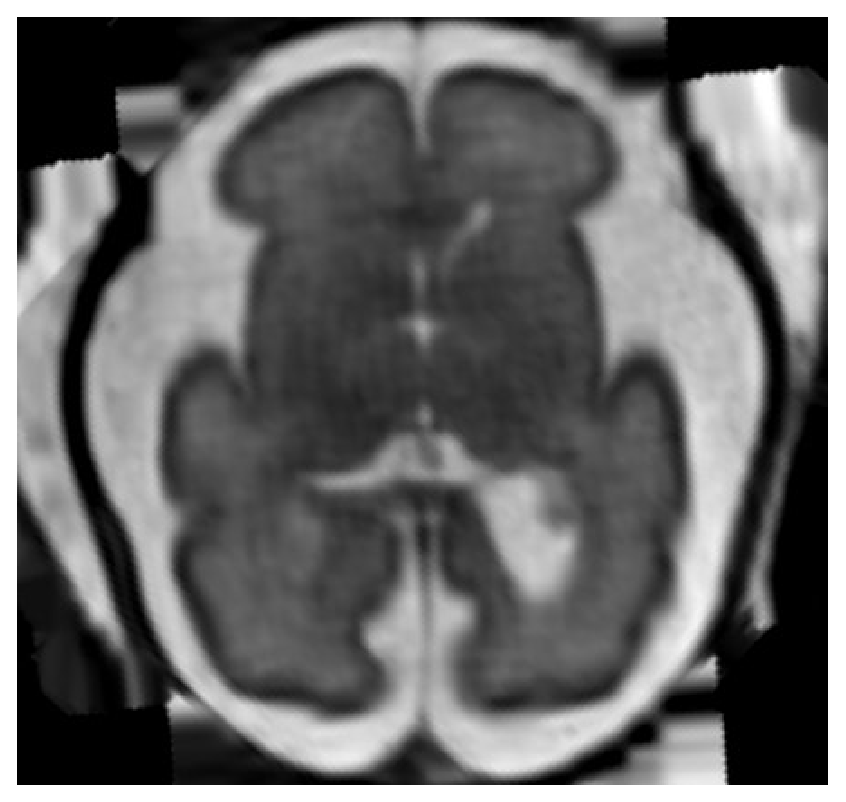
\includegraphics[width=0.3\columnwidth]{hr_axl.eps}&
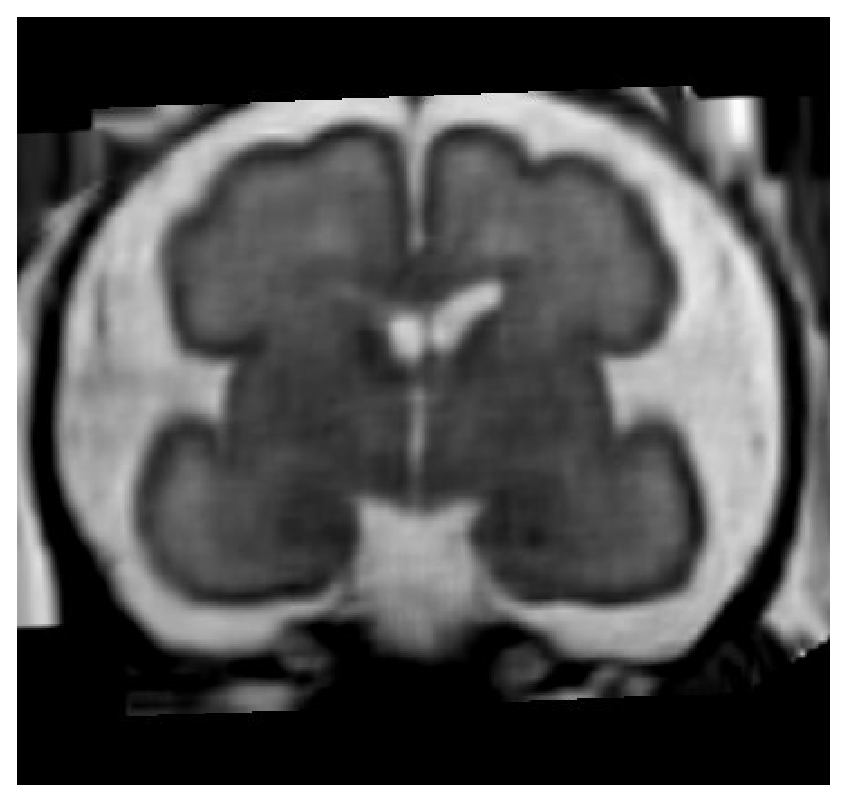
\includegraphics[width=0.3\columnwidth]{hr_cor.eps}&
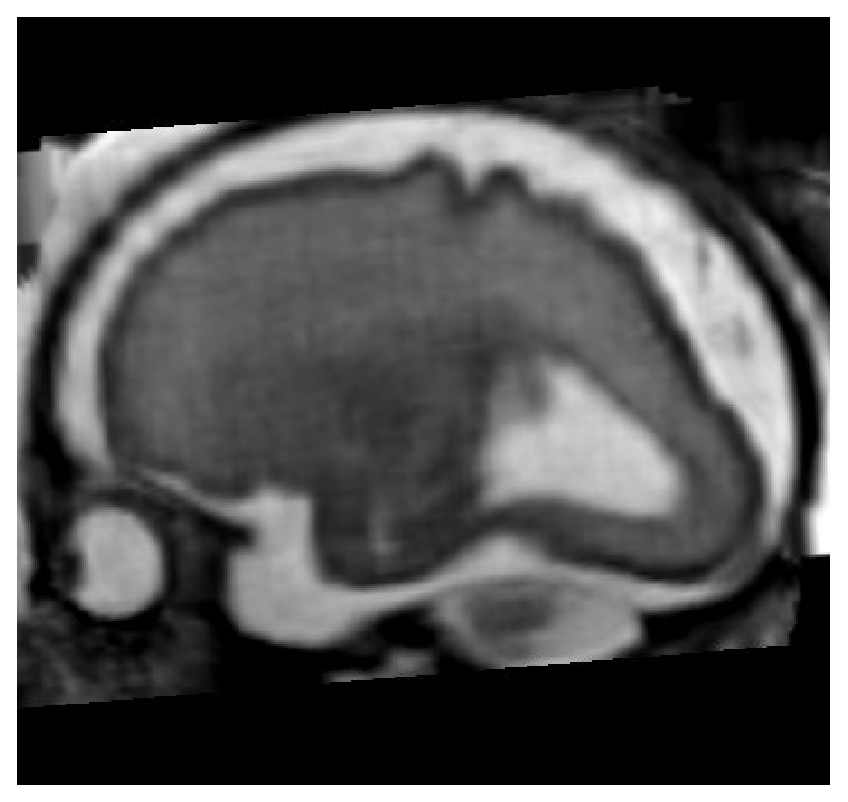
\includegraphics[width=0.3\columnwidth]{hr_sag.eps}\\
{(a)}&{(b)}&{(c)}\\
\end{tabular}
\caption{Example of an anatomical reconstruction of a fetal brain by using
\texttt{btkImageReconstruction}. (a) axial, (b) coronal, and (c) sagital view.}
\label{fig:reconstruction}
\end{figure}


\subsection{Tractography}

    \subsubsection*{Standard usage}
        Suppose you want to perform a tractography on a diffusion weighted MRI dataset. You should have a dwi image, the corresponding gradient vectors' coordinates, a mask of the brain white matter and a label image of the seeds. Assume this data is stored in files named repsectively for instance \texttt{data.nii.gz}, \texttt{data.bvec}, \texttt{mask.nii.gz} and \texttt{seeds.nii.gz}. The tractography is accomplished by the command below.
            \begin{quote}
                \texttt{btkTractography -d data.nii.gz -v data.bvec -m mask.nii.gz -l seeds.nii.gz}
            \end{quote}
        When the program terminates its task, the probability connection map and the fibers estimation are saved in files respectively named \texttt{map.nii.gz} and \texttt{fibers.vtk}. The connection map is a volume image of probability intensities (\texttt{i.e.} intensities between 0 and 1) with the same origin, orientation and spacing as the diffusion weighted image. The fibers are polygonal data of VTK library in world coordinates. The standard pipeline of the program is shown in Fig.~\ref{btkTractography-fig:standard-pipeline}.
            \begin{figure}
                \centering
                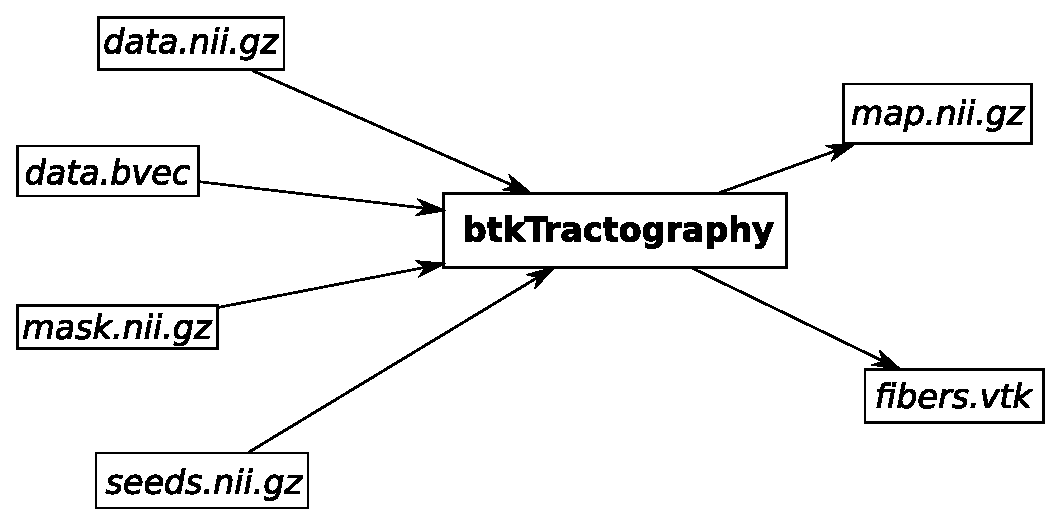
\includegraphics[width=0.6\textwidth]{btkTractographyPipeline}
                \caption{Standard pipeline of the btkTractography program.}
                \label{btkTractography-fig:standard-pipeline}
            \end{figure}

    \subsubsection*{Advanced usage}
        In addition to standard arguments of \texttt{btkTractography} program, there are some other parameters that let you to alter algorithm's behaviour. Since the default parameters values may work in the most of cases, they are optional. A list is of optional features is avaible by using the command
            \begin{quote}
                \texttt{btkTractography -\hspace{0.1mm}-help}
            \end{quote}
        and program's arguments are much more described below.

        \paragraph*{Model's order}
                \begin{table}
                    \centering
                    \caption{test}
                    \begin{tabular}{r|l}
                        \textbf{Action}  & modify model's order (\texttt{i.e.} spherical harmonics order)\\
                        \hline
                        \textbf{Default} & 4\\
                        \textbf{Command} & \texttt{-\hspace{0.1mm}-model-order <n>} \hfill \texttt{n}$\in\{2,4,6,8\}$
                    \end{tabular}
                \end{table}

        \paragraph*{Model's regularization}
            \begin{center}
                \begin{tabular}{rl}
                    \textbf{Action}  & modify the regularization coefficient of the model estimation\\
                    \textbf{Effect}  & reduce estimation errors\\
                    \textbf{Default} & 0.006\\
                    \textbf{Command} & \texttt{-\hspace{0.1mm}-model-regularization <r>} \hfill \texttt{r}$\in\mathbb{R}$
                \end{tabular}
            \end{center}

        \paragraph*{Displacement step size}
            \begin{center}
                \begin{tabular}{rl}
                    \textbf{Action}  & modify the displacement length of the particles in voxels\\
                    \textbf{Effect}  & control the displacement speed of the particles\\
                    \textbf{Default} & 0.5\\
                    \textbf{Command} & \texttt{-\hspace{0.1mm}-step-size <r>} \hfill \texttt{r}$\in\mathbb{R}_+^*$
                \end{tabular}
            \end{center}

            \begin{figure}
                \centering
                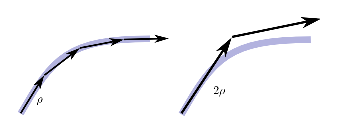
\includegraphics[height=0.1\textheight]{stepSize}
                \caption{}
            \end{figure}

        \paragraph*{Angular threshold}
            \begin{center}
                \begin{tabular}{rl}
                    \textbf{Action}  & modify the maximal angle in radians between two successive vectors\\
                    \textbf{Effect}  & constraint the curvature \emph{a priori} of the estimated fibers\\
                    \textbf{Default} & $\pi/3$\\
                    \textbf{Command} & \texttt{-\hspace{0.1mm}-angular-threshold <a>} \hfill \texttt{a}$\in]0,2\pi[$
                \end{tabular}
            \end{center}

            \begin{figure}
                \centering
                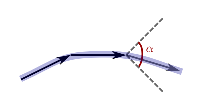
\includegraphics[height=0.1\textheight]{angleThreshold}
                \caption{}
            \end{figure}

        \paragraph*{Rigidity}
            \begin{center}
                \begin{tabular}{rl}
                    \textbf{Action}  & modify the concentration of the VMF use in the \emph{prior} density\\
                    \textbf{Effect}  & constraint the rigidity \emph{a priori} of the estimated fibers\\
                    \textbf{Default} & 30\\
                    \textbf{Command} & \texttt{-\hspace{0.1mm}-curve-constraint <r>} \hfill \texttt{r}$\in\mathbb{R}_+^*$
                \end{tabular}
            \end{center}

            \begin{figure}
                \centering
                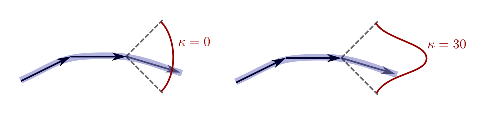
\includegraphics[height=0.1\textheight]{concentration}
                \caption{}
            \end{figure}

        \paragraph*{Number of particles}
            \begin{center}
                \begin{tabular}{rl}
                    \textbf{Action}  & modify the number of particles in th system\\
                    \textbf{Effect}  & control the algorithm's precision\\
                    \textbf{Default} & 1000\\
                    \textbf{Command} & \texttt{-\hspace{0.1mm}-number-of-particles <n>} \hfill \texttt{n}$\in\mathbb{N}^*$
                \end{tabular}
            \end{center}

        \paragraph*{Resampling threshold}
            \begin{center}
                \begin{tabular}{rl}
                    \textbf{Action}  & modify the effective sampling threshold (in \%)\\
                    \textbf{Effect}  & control the particles with a low weight\\
                    \textbf{Default} & 0.6\\
                    \textbf{Command} & \texttt{-\hspace{0.1mm}-resampling-threshold <r>} \hfill \texttt{r}$\in[0,1]$
                \end{tabular}
            \end{center}

